\chapter{Simulating Orbital Mechanics}
\section{Preface}
Text text text

\section{Relevant Physical and Mathetmatical Background}
\subsection{Classic Gravitational Force}
Already in the 17th century, \textit{Isaac Newton} formulated the gravitational force existing between any two objects with masses greater than zero. The strength of the force is given by the equation
\begin{equation}
    F = G\frac{m_{1}m_{2}}{r^{2}},
    \label{eq:force_gravity}
\end{equation}
where $m_{1}$ and $m_{2}$ are the respective masses of the two objects, $r$ is the distance between them, and $G$ is a the \textit{universal gravitational constant},
\begin{equation}
    G = \SI{6.6743(15)e-11}{\newton\metre\squared\per\kg\squared}
    \label{eq:universal_gravity_constant}
\end{equation}

The direction of the force is the line connecting the centers of mass of the two objects. Due to Newton's third law, the forces acting on the two objects are equal and opposite: the force applied by $m_{1}$ on $m_{2}$, $F_{1\to2}$, is pointing \textbf{from} $m_{2}$ \textbf{onto} $m_{1}$, and the force applied by $m_{2}$ on $m_{1}$, $F_{2\to1}$ is pointing \textbf{from} $m_{1}$ \textbf{onto} $m_{2}$ - and is exactly opposite to $F_{1\to2}$, i.e. in vector notation
\begin{equation}
    \vec{F}_{1\to2} = -\vec{F}_{2\to1}.
    \label{eq:gravity_force_vector_directions}
\end{equation}

If the two objects have positions $\vec{r}_{1}$ and $\vec{r}_{2}$, the vector pointing from object $1$ to object $2$ is
\begin{equation}
  \vec{r}_{1\to2} = \vec{r}_{2} - \vec{r}_{1},
  \label{eq:position_vector}
\end{equation}
with the vector pointing from object $2$ to object $1$ having the exact opposite components, i.e. $\vec{r}_{2\to1}=-\vec{r}_{1\to2}$. The norms of $\vec{r}_{1\to2}$ and $\vec{r}_{2\to1}$ are simply $r$ (the distance between the objects), and their directions are the unit vectors in the direction of $\vec{r}_{1\to2}$ and $\vec{r}_{2\to1}$, respectively:
\begin{align}
  \hat{r}_{1\to2} &= \frac{\vec{r}_{1\to2}}{\vnorm{r}_{1\to2}} = \frac{\vec{r}_{1\to2}}{r}\nonumber,\\
  \hat{r}_{2\to1} &= \frac{\vec{r}_{2\to1}}{\vnorm{r}_{2\to1}} = \frac{\vec{r}_{2\to1}}{r} = -\hat{r}_{1\to2}.
  \label{eq:normed_position_vector}
\end{align}

\begin{figure}
  \begin{center}
    \begin{tikzpicture}
      \pgfmathsetmacro{\a}{4}
      \pgfmathsetmacro{\b}{2}
      \coordinate (m1) at (0,0);
      \coordinate (m2) at (\a,\b);
      \coordinate (dp) at (-\b, \a);
      \coordinate (l1) at ($(m1)!1.3cm!(dp)$);
      \coordinate (l2) at ($(m2) + (m1)!1.3cm!(dp)$);
      \def\R{1cm}
      \def\r{0.5cm}
      \def\F{0.8cm}
      \draw[vector, xred, dashed] ($(m1)+(m1)!\R!(m2)$) -- ++($(m1)!\F!(m2)$) node[midway, below right, xshift=-1mm] {$\vec{F}_{2\to1}$};
      \draw[vector, xgreen, dashed] ($(m2)-(m1)!\r!(m2)$) -- ++($(m1)!-\F!(m2)$) node[midway, above left, xshift=1mm] {$\vec{F}_{1\to2}$};
      \draw[thick, fill=xgreen!50] (m1) circle (\R) node {$m_{1}$};
      \draw[thick, fill=xred!50] (m2) circle (\r) node {$m_{2}$};
      \draw[thick, cap=round, decorate, decoration={brace, amplitude=5pt}] (l1) -- (l2) node[midway, above left, xshift=0mm, yshift=2mm]{$r$};
      \draw[thick, densely dotted, black!75] ($(m1)+(m1)!0.15!(l1)$) -- (l1);
      \draw[thick, densely dotted, black!75] ($(m2)+(m1)!0.15!(l1)$) -- (l2);
    \end{tikzpicture}
  \end{center}
  \caption{Gravitational force between two objects with masses $m_{1}$ and $m_{2}$. Each object applies an attrctive force on the other object, with norm $F=G\frac{m_{1}m_{2}}{r^{2}}$ (where $r$ is the distance between the objects) and in the direction pointing from each object to the other object.}
  \label{fig:gravity_basics}
\end{figure}

In total, the vector notation of the gravitational force applied by the objects on each other are
\begin{align}
  \vec{F}_{1\to2} &= Gm_{1}m_{2}\frac{\hat{r}_{1\to2}}{r^{2}}\nonumber,\\
  \vec{F}_{2\to1} &= Gm_{1}m_{2}\frac{\hat{r}_{2\to1}}{r^{2}} = -\vec{F}_{1\to2}.
  \label{eq:gravity_forces_vector_notation}
\end{align}

\begin{note}{Another gravity force vector notation}{}
  In some textbooks, \autoref{eq:gravity_forces_vector_notation} are written without the unit vectors $\hat{r}_{1\to2}$ and $\hat{r}_{2\to1}$, instead using the distance vectors and dividing by $r^{3}$, i.e.
  \begin{align*}
    \vec{F}_{1\to2} &= Gm_{1}m_{2}\frac{\vec{r}_{1\to2}}{r^{3}},\\
    \vec{F}_{2\to1} &= Gm_{2}m_{1}\frac{\vec{r}_{2\to1}}{r^{3}}.
  \end{align*}
  The result is of course the same as in \autoref{eq:gravity_forces_vector_notation}, since for any non zero vector $\vec{v}$,
  \begin{align*}
    \frac{\vec{v}}{\vnorm{v}^{3}} = \frac{1}{\vnorm{v}^{2}}\frac{\vec{v}}{\vnorm{v}} = \frac{1}{\vnorm{v}^{2}}\hat{v}.
  \end{align*}
\end{note}

Let us look at an example of calculating the gravitational forces between two objects.

\begin{example}{Calculating a gravitational force}{grav_force_2_objects}
  Let us calculate the gravitational forces between two objects $A$ and $B$, using the following parameters:
  \begin{align*}
    \vec{r}_{A}&=\colvec{1;-2;0},\ m_{A} = 1,\\
    \vec{r}_{B}&=\colvec{2;5;-2},\ m_{B} = 2.
  \end{align*}
  For the sake of simplicity, we use $G=1$ and don't consider units with this example.

  The vector pointing from $A$ to $B$ is
  \[
    \vec{r}_{A\to B} = \vec{B}-\vec{A} = \colvec{2;5;-2} - \colvec{1;-2;0} = \colvec{1;7;-2},
  \]
  and the vector pointing from $B$ to $A$ is
  \[
    \vec{r}_{B\to A} = -\vec{r}_{A\to B} = \colvec{-1;-7;2}.
  \]

  The disntace $r$ between the objects is the norm of either of the above vectors, so we'll use $\vec{r}_{A\to B}$:
  \[
    r = \vnorm{r}_{A\to B} = \sqrt{1^{2}+7^{2}+2^{2}} = \sqrt{19} \approx 7.3485.
  \]

  The direction vectors are therefore
  \begin{align*}
    \hat{r}_{A\to B} &= \frac{1}{7.3485}\colvec{1;7;-2} = \colvec{0.1361;0.9526;-0.2722},\\
    \hat{r}_{B\to A} &= -\hat{r}_{A\to B} = \colvec{-0.1361;-0.9526;0.2722}.
  \end{align*}

  The gravity force which $A$ applies onto $B$ is then
  \[
    \vec{F}_{A\to B} = \cancel{G}\frac{\overbrace{m_{1}m_{2}}^{=2\times1}}{r^{2}}\hat{r}_{A\to B} = \frac{2}{54}\colvec{0.1361;0.9526;-0.2722} = \colvec{0.0050;0.0353;-0.101}.
  \]
  and similarily,
  \[
    \vec{F}_{B\to A} = -\vec{F}_{A\to B} = \colvec{-0.0050;-0.0353;0.101}.
  \]
\end{example}

In the case where we only consider two objects, and choose our frame of reference such that one of the objects is stationary - an analytical solution to the spatial trajectory taken by the second object is known and well studied. It is called a \textbf{Keplerian orbit}, and it always takes the form of a conic section. Let us take a short detour to discuss conic sections.

\subsection{Conic Sections}
A conic section (sometimes simply just called \enquote{a conic}) is a 2-dimensional shape resulting from the intersection of a plane and a cone (see \autoref{fig:3d_conic_1}). Depending on the angle $\alpha$ by which the plane intersects the cone relative to the the cone's side, the resulting shape can be one of 3 general types (here $\theta$ is the cone's angle):
\begin{enumerate}
  \item If $\alpha>\theta$ the intersection is an \textbf{ellipse}. If in addition $\alpha=\ang{90}$ the ellipse becomes a \textbf{circle}.
  \item If $\alpha=\theta$ the intersection is a \textbf{parabola}.
  \item If $\alpha<\theta$ the intersection is a \textbf{hyperbola}.
\end{enumerate}

\begin{figure}
  \begin{center}
    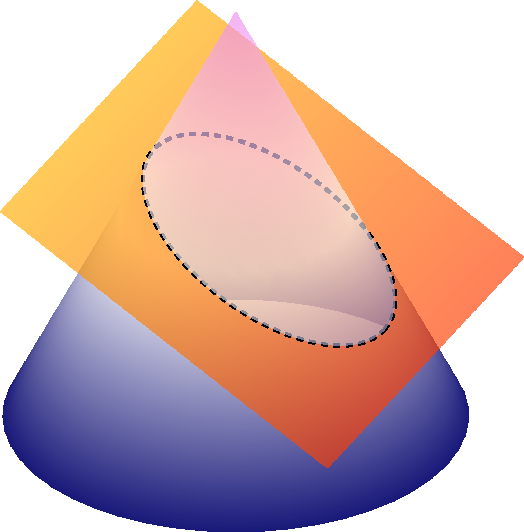
\includegraphics[scale=0.65]{figs/mechanics/cone_plane_3d.pdf}
  \end{center}
  \caption{An intersection of a cone and a plane. Both the cone and plane are infinite - the cone extends infinitely \enquote{down}, but also has a second \enquote{inverted} part on the top, also extending to infinity. In the case here shown, the intersection is an ellipse. Image reproduced with modifications from !SOURCE!} % source: https://latexdraw.com/draw-a-plane-intersecting-a-cone-in-latex/
  \label{fig:3d_conic_1}
\end{figure}

\begin{figure}
  \begin{center}
    \begin{tikzpicture}
      \pgfmathsetmacro{\Lth}{1}
      \pgfmathsetmacro{\x}{2.25}
      \pgfmathsetmacro{\y}{3.5}
      \pgfmathsetmacro{\th}{atan(\y/\x)}
      \coordinate (h1) at (0,0);
      \coordinate (h2) at (0,-\y);

      % Cone
      \draw[filledangle={xpurple}] (h1) -- (0,-\Lth) arc (-90:-\th:\Lth) node [above, pos=0.37] {$\theta$};
      \draw[thick] (h1) -- (\x,-\y);
      \draw[thick] (h1) -- (-\x,-\y);
      \draw[thick, dashed, black!75] (-\x,-\y) -- ($(-\x,-\y)!1.4!(h1)$);
      \draw[thick] (-\x,-\y) -- ($(-\x,-\y)!1.2!(h1)$) node[above left, pos=0.6] {$C$};
      \draw[thick, dashed, black!75] (\x,-\y) -- ($(\x,-\y)!1.4!(h1)$);
      \draw[thick] (\x,-\y) -- ($(\x,-\y)!1.2!(h1)$);
      \draw[thick, dashed, black!75] (0,-\y) -- ($(0,-\y)!1.25!(h1)$) node[right, pos=0.05] {$h$};

      % Plane
      \pgfmathsetmacro{\px}{2}
      \pgfmathsetmacro{\pya}{1.25}
      \pgfmathsetmacro{\pyb}{2.25}
      \pgfmathsetmacro{\alph}{atan((\pyb-\pya)/(2*\px))}
      \pgfmathsetmacro{\Lalph}{0.75}
      \coordinate (p1) at (-\px,-\pya);
      \coordinate (p2) at (\px,-\pyb);
      \draw[thick, xred, dashed] (p1) -- ($(p1)!-0.2!(p2)$);
      \draw[thick, xred, dashed] (p2) -- ($(p1)!1.2!(p2)$);
      \draw[thick, xred, name path=p1--p2] (p1) -- (p2) node[above, pos=0.95] {$P$};
      \draw[name path=h1--h2, opacity=0] (h1) -- (h2);
      \path[name intersections={of=p1--p2 and h1--h2, by=E}];
      \draw[filledangle={xblue}] (E) -- ++(0,-\Lalph) arc (-90:-\alph:\Lalph) node[above, pos=0.35] {$\alpha$};
    \end{tikzpicture}
  \end{center}
  \caption{Side view of an infinite cone $C$ and an infinite plane $P$ intersecting it. The angle between $P$ and the cone's height line $h$ is $\alpha$, and the angle between the cone's surface and $h$ is $\theta$. In this figure $0<\theta<\alpha<\ang{90}$, and thus the shape formed by the intersection of $C$ and $P$ is an ellipse.}
  \label{fig:cone_side_view}
\end{figure}


Depending on the exact parameters of both $C$ and $P$, the resulting conic section can be \textbf{degenerate} - either a point, a line or two intersection lines. This happens if $P$ goes throgh the vertex point of $C$: if $\alpha=\ang{90}$ the result is a single point \footnote{one can understand this as being a circle with radius $r=0$.}, if $\alpha=\theta$ the result is a single line, and if $\alpha>\theta$ the result is two intersecting lines.

\subsubsection{Geometric Properties of Conic Sections}
Of the non-degenerate conic sections, the ellipse is the only closed curve. Both the parabola and hyperbola are open: in essence, this means that they diverge to infinity. A common geometric definition for all conic sections is the following: given a line $L$ (called the \textbf{directrix}) and a point $F$ (called the \textbf{locus}), a conic section is the set $C$ of all points $\left\{p\right\}$ for which the distance $Fp$ is equal to a constant multiple of the distance $Lp$:
\begin{equation}
  C = \left\{ p \mid \snorm{Fp} = e\snorm{Lp} \right\}.
  \label{eq:conic_section_geometric_definition}
\end{equation}
The constant $e$ is called the \textbf{eccentricity} of the conic section.

\begin{figure}
  \begin{center}
    \begin{tikzpicture}
    \begin{axis}[
      graph2d,
      width=12cm, height=12cm,
      xmin=-2, xmax=2,
      ymin=-2, ymax=2,
      restrict y to domain=-3:3,
      xticklabels={,},
      yticklabels={,},
      cycle list/Spectral,
      declare function={
        conic(\x,\A,\E) = \A*(\E+\A)/(1+\E*cos(\x));
      },
    ]
      \pgfmathsetmacro{\A}{0.5}
      \foreach \E in {0.0,0.1,...,5,5.5,...,10} { 
        \edef\drawconic{\noexpand\addplot[black!5, very thick, data cs=polar, domain=0:2*pi, samples=100, smooth] (x,{conic(x,\A,\E)});}
          \drawconic
        }
      \foreach \E in {0,0.25,...,1,2,...,5} { 
        \edef\drawconic{\noexpand\addplot+[very thick, data cs=polar, domain=0:2*pi, samples=100, smooth] (x,{conic(x,\A,\E)});}
          \drawconic
        }
      % \addplot[function={xred}] ()
    \end{axis}
    \end{tikzpicture}
  \end{center}
  \caption{Several conic sections with different eccentricities $\left\{e_{i}\right\}$ and the same locus $F$ and directrix $L$. (NOTE: figure still WIP)}
  \label{fig:conic_sections_geometrically}
\end{figure}

MORE TEXT HERE

\subsubsection{Cartesian coefficients}
All conic sections can be expressed as the solutions to the following general equation in $\Rs[2]$:
\begin{equation}
  Ax^{2}+Bxy+Cy^{2}+Dx+Ey+F=0,
  \label{eq:conic_section_cartesian_form}
\end{equation}
where $A, B, C, D, E, F$ are all real coefficients such that $A, B$ and $C$ are all nonzero. The above equation can be written in matrix form as
\begin{equation}
  \rowvec{x;y;1}
  \begin{bmatrix}
    A   & B/2 & D/2 \\
    B/2 &   C & E/2 \\
    D/2 & E/2 &   F
  \end{bmatrix}
  \colvec{x;y;1}=0.
  \label{eq:conic_section_cartesian_form_matrix}
\end{equation}

In this form, the different typs of conic sections arise from the sign of the term
\begin{equation}
  \Delta = B^{2}-4AC,
  \label{eq:conic_section_discriminant}
\end{equation}
called the \textbf{discriminent} of the conic equation, as following:
\begin{enumerate}
  \item If $B^{2}-4AC<0$ the equation represents an ellipse. If in addition $A=C$ and $B=0$ the discriminent collapses to $-A^{2}$ - which represents a circle.
  \item If $B^{2}-4AC=0$, the equation represents a parabola.
  \item If $B^{2}-4AC>0$, the equation represents a hyperbola.
\end{enumerate}

Note that the discriminent can be represented as a $2\times2$ determinant derived from the matrix form of the Cartesian coefficients:
\begin{equation}
  \Delta = -4\begin{vmatrix} A & B/2 \\ B/2 & C \end{vmatrix}.
  \label{eq:conic_section_discriminant_as_determinant}
\end{equation}

\subsubsection{Conic Section From 5 Points}
If we know 5 points lying on a conic,
\begin{equation}
  \begin{cases}
    \bm{p}_{1}=\left(x_{1},y_{1}\right)\\
    \bm{p}_{2}=\left(x_{2},y_{2}\right)\\
    \vdots\\
    \bm{p}_{5}=\left(x_{5},y_{5}\right),
  \end{cases}
  \label{eq:5_points_on_conic}
\end{equation}
we can determine all the conic Cartesian coefficients by solving the equation
\begin{equation}
  \begin{bmatrix}
    x_{1}^{2} & x_{1}y_{1} & y_{1}^{2} & x_{1} & y_{1} & 1\\
    x_{2}^{2} & x_{2}y_{2} & y_{2}^{2} & x_{2} & y_{2} & 1\\
    x_{3}^{2} & x_{3}y_{3} & y_{3}^{2} & x_{3} & y_{3} & 1\\
    x_{4}^{2} & x_{4}y_{4} & y_{4}^{2} & x_{4} & y_{4} & 1\\
    x_{5}^{2} & x_{5}y_{5} & y_{5}^{2} & x_{5} & y_{5} & 1
  \end{bmatrix}
  \colvec{A;B;C;D;E;F} = \colvec{0;0;0;0;0},
  \label{eq:5_points_determine_conic_matrix_equation}
\end{equation}
which can be done by finding the null space of the matrix in the above equation.

\subsubsection{Some More About Ellipses}
Unlike the other conic sections, an ellipse has two focus points (simply called its \textbf{foci}): $F_{1}$ and $F_{2}$. One of these always corresponds to the conic section definition of the focus. In an ellipse, the sum of the distances from any point to the two foci is always constant. In a sense, an ellipse is an elognated circle: instead of having a single radius, it has two orthogonal \textbf{axes}: the semi-major axis $a$ and the semi-minor axis $b$ (such that $a\geq b$).

\begin{figure}
  \begin{center}
    \begin{tikzpicture}
      \pgfmathsetmacro{\a}{5.5}
      \pgfmathsetmacro{\b}{3.5}
      \pgfmathsetmacro{\c}{\a*sqrt(1-(\b/\a)^2)}

      % Drawings
      \draw[ultra thick, xred] (0,0) ellipse [x radius=\a, y radius=\b];
      \node[point={}] (C) at (0,0) {};
      \node[point={}] (pa1) at (\a,0) {};
      \node[point={}] (pa2) at (-\a,0) {};
      \node[point={}] (pb1) at (0,\b) {};
      \node[point={}] (pb2) at (0,-\b) {};
      \draw[thick, dashed, black!75] (pa1) -- (pa2);
      \draw[thick, dashed, black!75] (pb1) -- (pb2);
      \draw[ultra thick, xgreen] (C) -- (pb1) node[midway, below, rotate=90] {semi-minor axis, $b$};
      \node[point={$F_{1}$}] (F1) at (\c,0) {};
      \node[point={$F_{2}$}] (F2) at (-\c,0) {};
      \draw[ultra thick, xpurple] (F2) -- (C) node[pos=0.5, below] {linear eccentricity, $l$};
      \draw[ultra thick, xblue] (C) -- (pa1) node[midway, below] {semi-major axis, $a$};
    \end{tikzpicture}
  \end{center}
  \caption{Some common geometric properties of an ellipse. NOTE: figure still WIP}
  \label{fig:ellipse_geometerically}
\end{figure}

The two foci are at a distance of $c=\sqrt{a^{2}-b^{2}}$ away from the center of the ellipse, a measure that also called \textbf{linear eccentricity}. The eccentricity of the ellipse is
\begin{equation}
  e = \frac{c}{a} = \frac{\sqrt{a^{2}-b^{2}}}{a} = \sqrt{1-\frac{b^{2}}{a^{2}}}.
  \label{eq:label}
\end{equation}

As mentioned already, in the case of a circle $e=0$, and we get that $c=0$ and that $\sqrt{1-\frac{b^{2}}{a^{2}}}=0$, i.e. $a=b$. The first equality means that the foci are located at the center of the ellipse, and the second equality means that the semi-major and semi-minor axes of the ellipse are the same. This is exactly what we excpect for a circle.

% more text: https://mathworld.wolfram.com/ConicSection.html

\subsection{Orbital Shapes}
Back from our short detour, we can now discuss the Keplerian orbits in more details. Suppose there are two objects: the first has mass $m_{1}$, and second mass $m_{2}$. For simplicity we will assume that $m_{1}\gg m_{2}$, such that we can assume it is stationary, while the second object experiences the Keplerian orbit - consider for example a satellite orbiting the earth. We will indeed from now on refer to the first (more massive) object simply as the \enquote{massive object}, and the second object as the \enquote{satellite}.

Although space is 3-dimensional, a Keplerian orbit is always 2-dimensional - since as mentioned before, it is always a conic section. The plane on which the orbit takes place, the \textbf{orbital plane}, is determined by the direction of velocity of the satellite and the direction connecting the centers of mass of the massive object and the satellite. The massive object is found at the locus of the conic section. The relative values of $m_{1}$ and the angular momentum of the satellite determine the eccentricity of the orbit.

For now, let us concentrate on an elliptic orbit, i.e. where $0\leq e < 1$. As mentioned, in such an orbit the massive object is at the locus of the ellipse, which is one of its foci - we will call it $F_{1}$ here. The point of closest to $F_{1}$ on the elliptical orbit is called the \textbf{periapsis} and denoted $r_{p}$. The point directly opposite $r_{p}$, i.e. the point closest to the second focus $F_{2}$ of the ellipse and furthest away from $F_{1}$ is called the \textbf{apoapsis}, denoted $r_{a}$ (\autoref{fig:terms_elliptical_orbit}). The direction from $F_{1}$ to the periapsis point is (unsuprisingly) called the \textbf{direction of periapsis}.

\begin{figure}
  \begin{center}
    \begin{tikzpicture}
      \pgfmathsetmacro{\a}{4}
      \pgfmathsetmacro{\b}{3}
      \pgfmathsetmacro{\c}{\a*sqrt(1-(\b/\a)^2)}

      % Drawings
      \draw[ultra thick, black!50] (0,0) ellipse [x radius=\a, y radius=\b];
      \node[point={center of orbit}] (C) at (0,0) {};
      \node[point={Perihelion}, rotate=-90] (pa1) at ({\a},0) {};
      \node[point={Aphelion}, rotate=90] (pa2) at (-\a,0) {};
      \node[point={}, fill=xblue, minimum size=7pt] (F1) at (\c,0) {};
      \node[point={$F_{2}$}] (F2) at (-\c,0) {};
      \node[draw=xblue, thick, fill=white, rounded corners, above left of=F1, xshift=-4mm, yshift=4mm, text=xblue] (F1txt) {Massive object at $F_{1}$};
      \draw[-stealth, thick, xblue] (F1txt) to [out=-90,in=90] (F1);
      \draw[xred, thick, cap=round, dashed, decorate, decoration={brace, amplitude=3pt, raise=5pt, mirror}] (\c,0) -- (pa1) node[midway, below, yshift=-2mm]{$r_{p}$};
      \draw[xdarkgreen, thick, cap=round, dashed, decorate, decoration={brace, amplitude=3pt, raise=5pt, mirror}] (pa2) -- (\c,0) node[midway, below, yshift=-2mm]{$r_{a}$};
    \end{tikzpicture}
  \end{center}
  \caption{Common terms in elliptical orbits.}
  \label{fig:terms_elliptical_orbit}
\end{figure}

The relation between the eccentricity of the orbit and the two distances $r_{p},r_{a}$ is
\begin{equation}
  e = \frac{r_{a}-r_{p}}{r_{a}+r_{p}} = 1-\frac{2}{\frac{r_{a}}{r_{p}}+1}.
  \label{eq:eccentricity_relation_to_apsis_1}
\end{equation}
Conversly, we can write the above relation as
\begin{equation}
  \frac{r_{a}}{r_{p}} = \frac{1+e}{1-e}.
  \label{eq:eccentricity_relation_to_apsis_2}
\end{equation}

\begin{example}{Earth's orbit around the sun}{}
  In the sun-earth system, where the sun is the massive object and the earth is the satellite, the periapsis distance is $r_{p}=\SI{1.47098450e+11}{\meter}$, and the apoapsis distance is $r_{a}=\SI{1.52097597e+11}{\meter}$. Therefore, the orbital eccentricity of Earth's orbit around the sun is about
  \begin{align*}
    e &= 1-\frac{2}{\frac{r_{a}}{r_{p}}+1} = 1-\frac{2}{\frac{1.52097597}{1.47098450}+1}\\
      &= 1-\frac{2}{1.033985+1} = 1-\frac{2}{2.033985}\\
      &= 1-0.983291 = 0.016709.
  \end{align*}
  This is a pretty round orbit (not a scientific term). 
\end{example}

At any point in a spatial trajectory, the velocity of the object in motion is always tangent to the trajectory it traces.  In the case of a Keplerian orbit, the angle between the direction of periapsis and the line connecting $F_{1}$ and the position of the satellite $r(t)$ at some given time $t$ is called the \textbf{true anomaly}, denoted as $\theta$.

\begin{figure}
  \begin{center}
    \begin{tikzpicture}
      \pgfmathsetmacro{\a}{3.5}
      \pgfmathsetmacro{\b}{3}
      \pgfmathsetmacro{\e}{sqrt(1-(\b/\a)^2)}
      \newcommand{\E}{47}
      \pgfmathsetmacro{\L}{1}

      % Drawings
      \draw[ultra thick, black!50] (0,0) ellipse [x radius=\a, y radius=\b];
      \node[point={}, fill=xdarkgreen, minimum size=10pt] (F1) at ({\a*\e},0) {};
      \draw[thick, black!75] (F1) -- (\a,0);
      \coordinate (r) at ({\a*cos(\E)},{\b*sin(\E)});
      \pgfmathsetmacro{\th}{atan(sin(\E)*sqrt(1-\e^2)/(cos(\E)-\e))}
      \draw[filledangle={xpurple}] (F1) -- ++(\L,0) arc (0:\th:\L) -- (F1); % why cycle doesn't work here? weird
      \pgfmathsetmacro{\XVA}{\L/2*cos(\th/2)}%
      \pgfmathsetmacro{\YVA}{\L/2*sin(\th/2)}%
      \node[xpurple] at ($(F1)+(\XVA,\YVA)$) {$\theta$};

      \pgfmathsetmacro{\dP}{180+atan(-\b/(\a*tan(\E)))}
      \draw[vector={xblue}] (r) -- ++(\dP:1cm) node[midway, above right] {$\vec{v}(t)$};
      \draw[xblue, very thick, dashed] (r) -- ++(\dP:-2cm);
      \draw[vector={xred}, very thick] (F1) -- (r) node[point={}] {};
      \node[below left=of r, xshift=8mm, yshift=5mm, xred] {$\vec{r}(t)$};
    \end{tikzpicture}
  \end{center}
  \caption{Position $\vec{r}$, velocity $\vec{v}$ and true anomaly $\theta$ in an elliptic orbit. Notice how the velocity is tangent to the trajectory.}
  \label{fig:magnitudes_elliptical_orbit}
\end{figure}

% TO WRITE: orbital constants and the vis-viva equation from energy conservation.
% TO WRITE: orbital equation.

% In general, Keplerian trajectories have some scalar and vector constants - i.e. quantities that are conserved throughout the orbit. The first is the \textbf{standard gravitational parameter} $\mu$, which is the universal gravitational constant $G$ times the total mass of the two objects:
% \begin{equation}
%   \mu = G\left(m_{1}+m_{2}\right),
% \end{equation}
% which in practice is approximately just
% \begin{equation}
%   \mu \approx Gm_{1},
%   \label{eq:standard_gravitational_parameter}
% \end{equation}
% since $m_{1}\gg m_{2}$.
%
% The second constant is the \textbf{specific relative angular momentum} of the sattelite, denoted $\bm{h}$. It is the cross product of the position vector of the sattelite at some time $\tau$, and its velocity at the same time:
% \begin{equation}
%   \bm{h} = \vec{r}\times\vec{v}.
%   \label{eq:specific_relative_angular_momentum}
% \end{equation}
% \begin{note}{Angular momentum is not a vector}{}
%   Since angular momentum in general is defined via the cross product, it is not a vector but a \textbf{pseudovector}. Therefore, it does not denoted using the vector symbol and instead is denoted by a bold-face letter. However, for the sake of simplicity we will consider it as a vector, since in $\Rs[3]$ vectors and pseudovectors behave very similarly. To better understand the concept of pseudo-vectors it is recommended to learn \textbf{geometrical algebra} (also sometimes called \textbf{Clifford algebra}). !SOURCE!
% \end{note}
%
% The third constant is the \textbf{specific orbital energy} $\varepsilon$. It is defined by the \textbf{vis-viva equation} using the kinetic energy $\varepsilon_{k}$ and potential energy $\varepsilon_{u}$:
% \begin{equation}
%   \varepsilon = \varepsilon_{k}+\varepsilon_{u} = \frac{v^{2}}{2} - \frac{\mu}{r},
%   \label{eq:vis-viva}
% \end{equation}
% where $v$ is the speed (norm of the velocity) of the satellite at any time $t'$, and $r$ is the distance to the massive object at the same time $t'$. Another form for this same energy is
% \begin{equation}
%   \varepsilon = -\frac{\mu}{2a},
%   \label{eq:vis-viva2}
% \end{equation}
% where here $a$ is the semi-major axis of the trajectory.
%
% We can use the above constants to calculate some conditions for the shape of the trajectory. For example - when it is expected to be perferctly circular. This happens when $e=0$. By solving \autoref{eq:vis-viva} for $v$ we get
% \[
%   \frac{v^{2}}{2} = \varepsilon+\frac{\mu}{r} = -\frac{\mu}{2a} + \frac{\mu}{r}.
% \]
% For a circular orbit $a=r$, and the above equation becomes
% \[
%   \frac{v^{2}}{2} = -\frac{\mu}{2r} + \frac{\mu}{r} = -\frac{\mu}{2r} + \frac{2\mu}{2r} = \frac{\mu}{2r},
% \]
% i.e.
% \begin{equation}
%   v = \sqrt{\frac{\mu}{r}} = \sqrt{\frac{Gm_{1}}{r}}.
%   \label{eq:speed_circular_orbit}
% \end{equation}
%
% In perfect circular motion we know that the total force acting on the object in motion is directed into the center of motion, is always orthogonal to its velocity and has a magnitude of exactly
% \begin{equation}
%   F = m\frac{v^{2}}{r}.
%   \label{eq:force_circular_motion}
% \end{equation}
%
% We can bring \autoref{eq:speed_circular_orbit} to the form of \autoref{eq:force_circular_motion} by raising $v$ to the second power, multiplying by $m_{2}$ and dividing by the radius. Its right hand side would then be
% \[
%   F = \frac{m_{2}}{r}\frac{Gm_{1}}{r} = G\frac{m_{1}m_{2}}{r^{2}},
% \]
% exactly the form of the gravitational force. This confirms \autoref{eq:speed_circular_orbit}.

\subsubsection{Calculating the precise trajectory from known magnitudes}
To get a precise projected trajectory for a satellite with known velocity $\vec{v}$ and position $\vec{r}$ around a massive object of known mass $M$ we can use the following steps:
\begin{enumerate}
  \item Calculate the standard gravitational parameter $\mu$ (REF) and the specific angular momentum vector $\vec{h}$ (REF). The eccentricity vector can then be calculated using (REF).
  \item If $\vnorm{e}<1$, the orbit is elliptical and we can proceed. If not - MORE TEXT?
  \item \ldots
\end{enumerate}

\subsection{Multiple Objects}

\section{Integration Methods}
\subsection{Euler Method}
% \subsubsection{Forward Method}
% \subsubsection{Backward Method}
% \subsubsection{Central Method}

\subsection{Verlet Integration}

\subsection{Runge-Kutta Method}
